\chapter{Appendix}
%
\begin{figure}[h]%
    \centering
    \subfloat[Reference pulse at CH1. The delayed pulse is fed to CH2.\label{subfig:osci:ch1-ch2_delayed_pulse}]
    {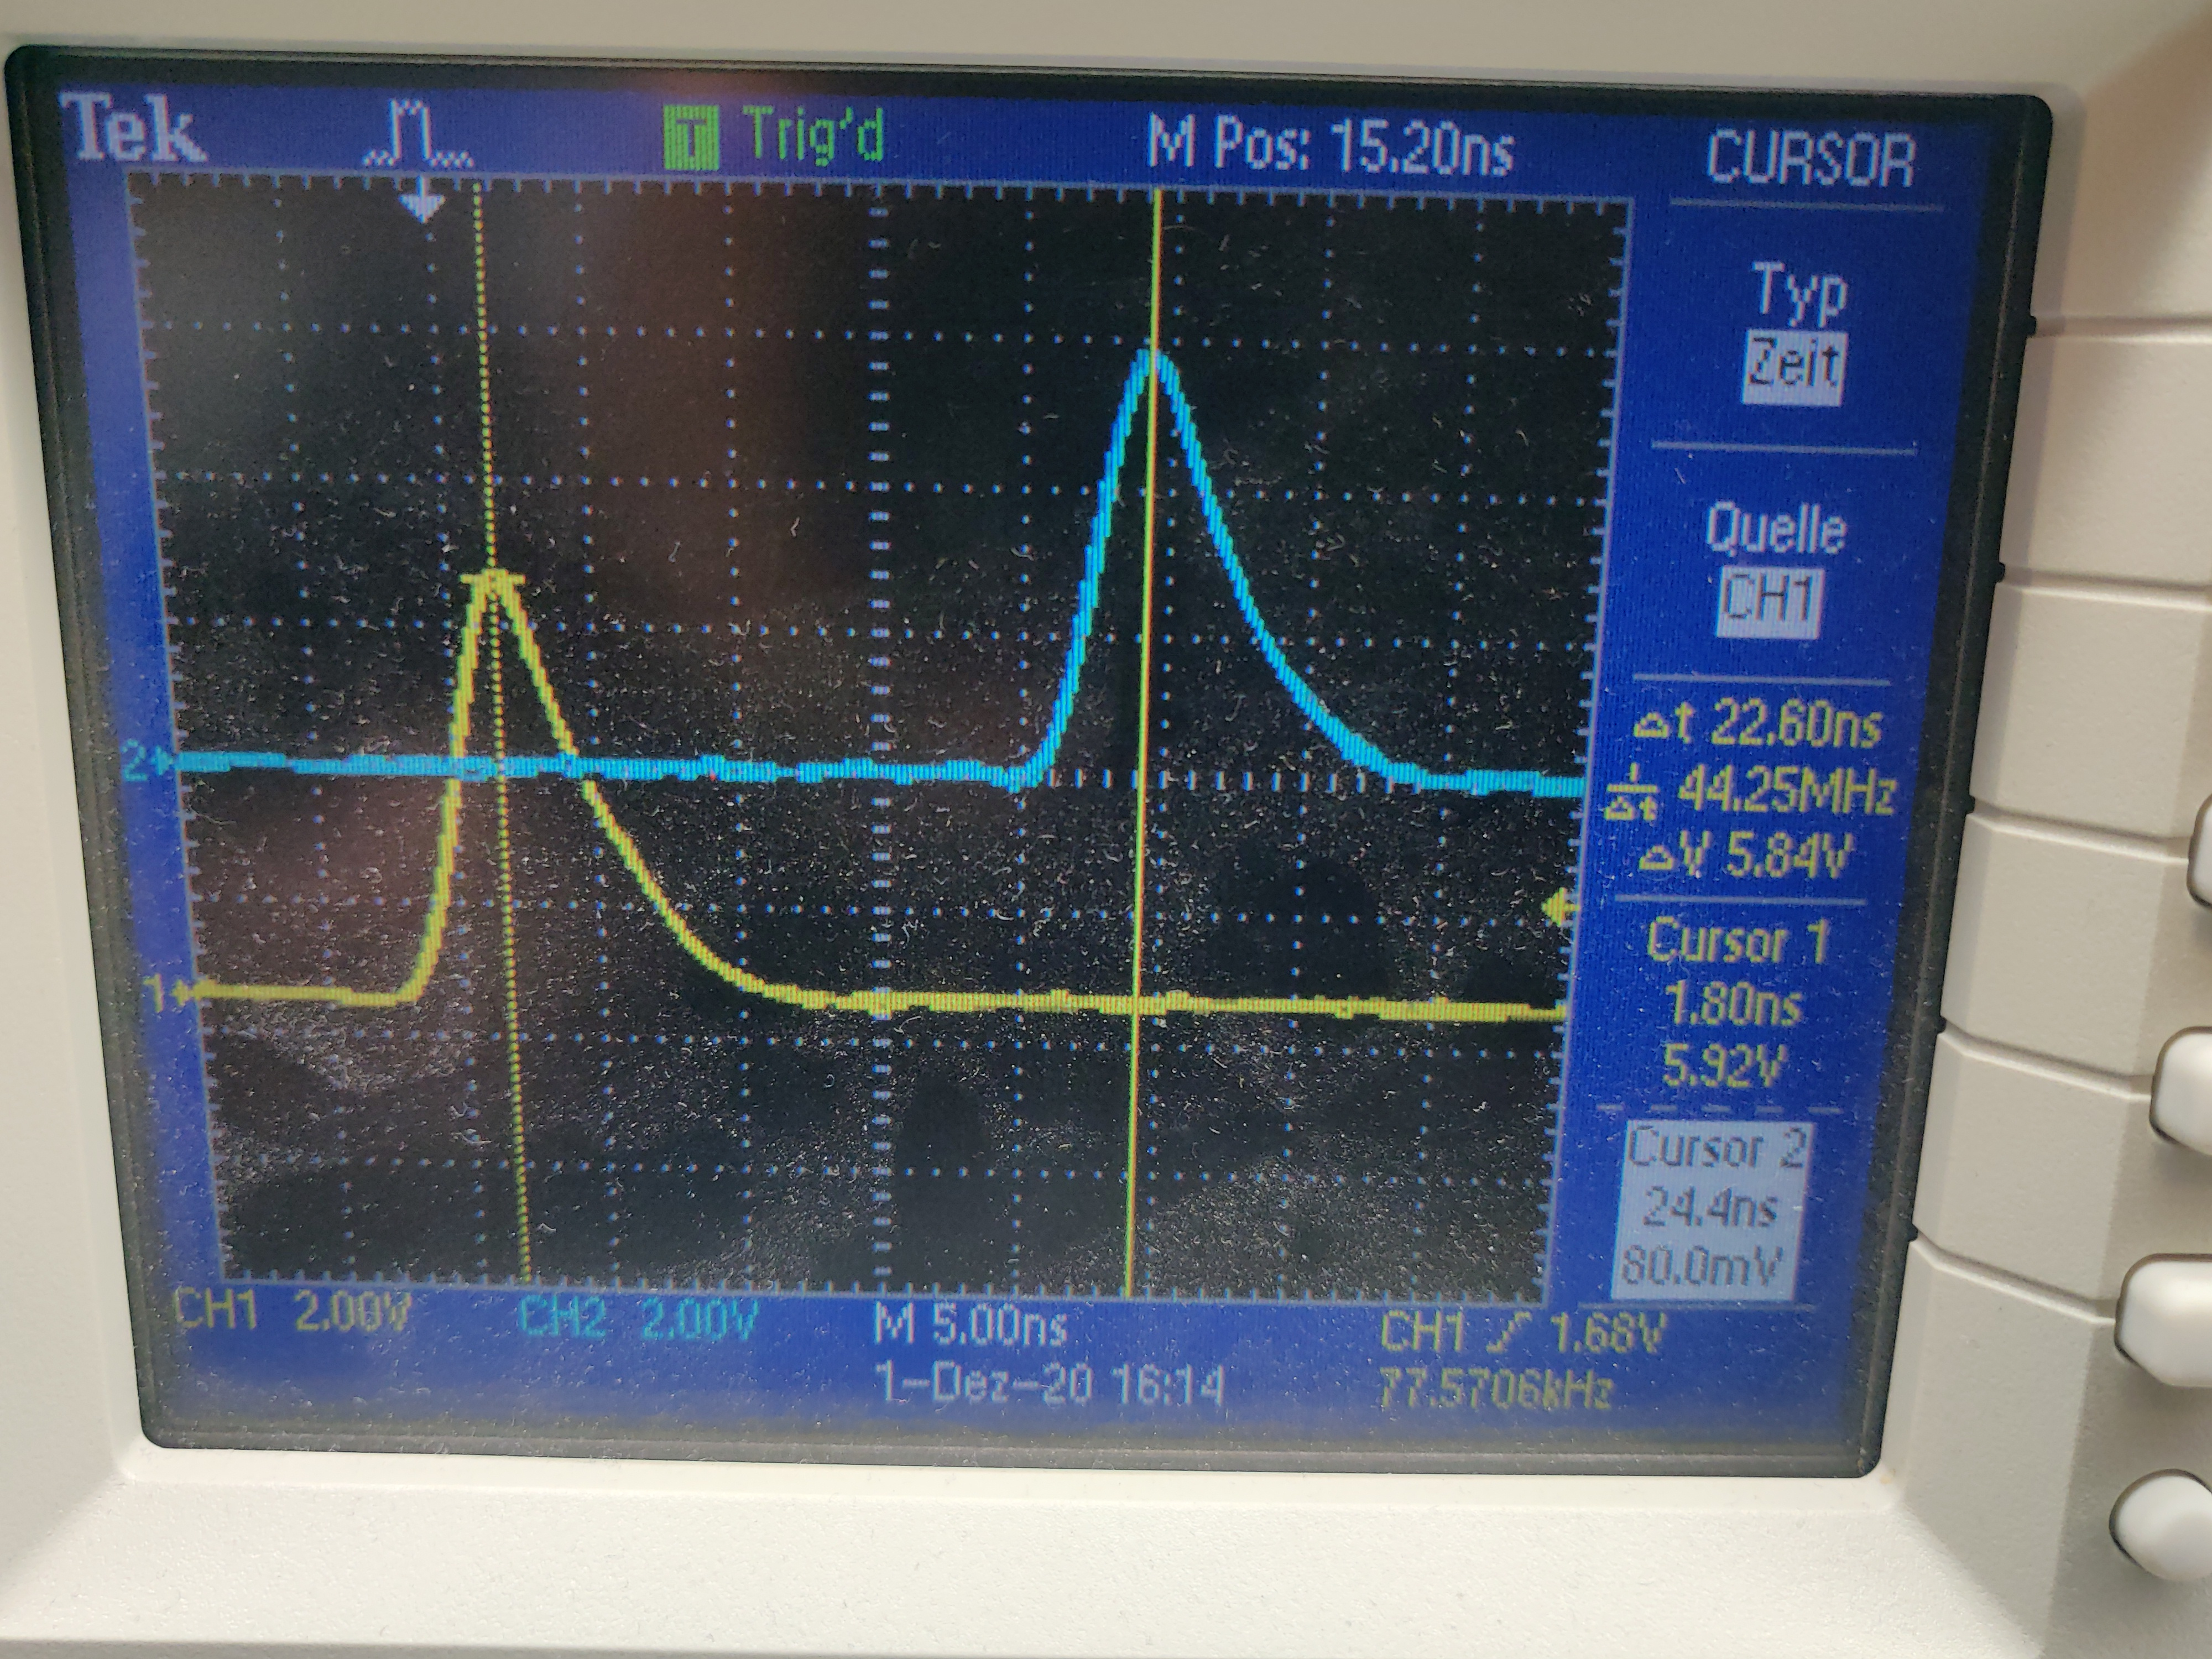
\includegraphics[width=0.45\linewidth]{messdaten/3-3-1_propagationDelay.jpg}}%
    \hspace{.05\linewidth}
    \subfloat[The reference pulse gets reflected at an open-ended cable connected to the same channel. A difference in time due to a finite propagation speed can be observed.\label{subfig:osci:3-3-2_open_reflectionTime}]
    {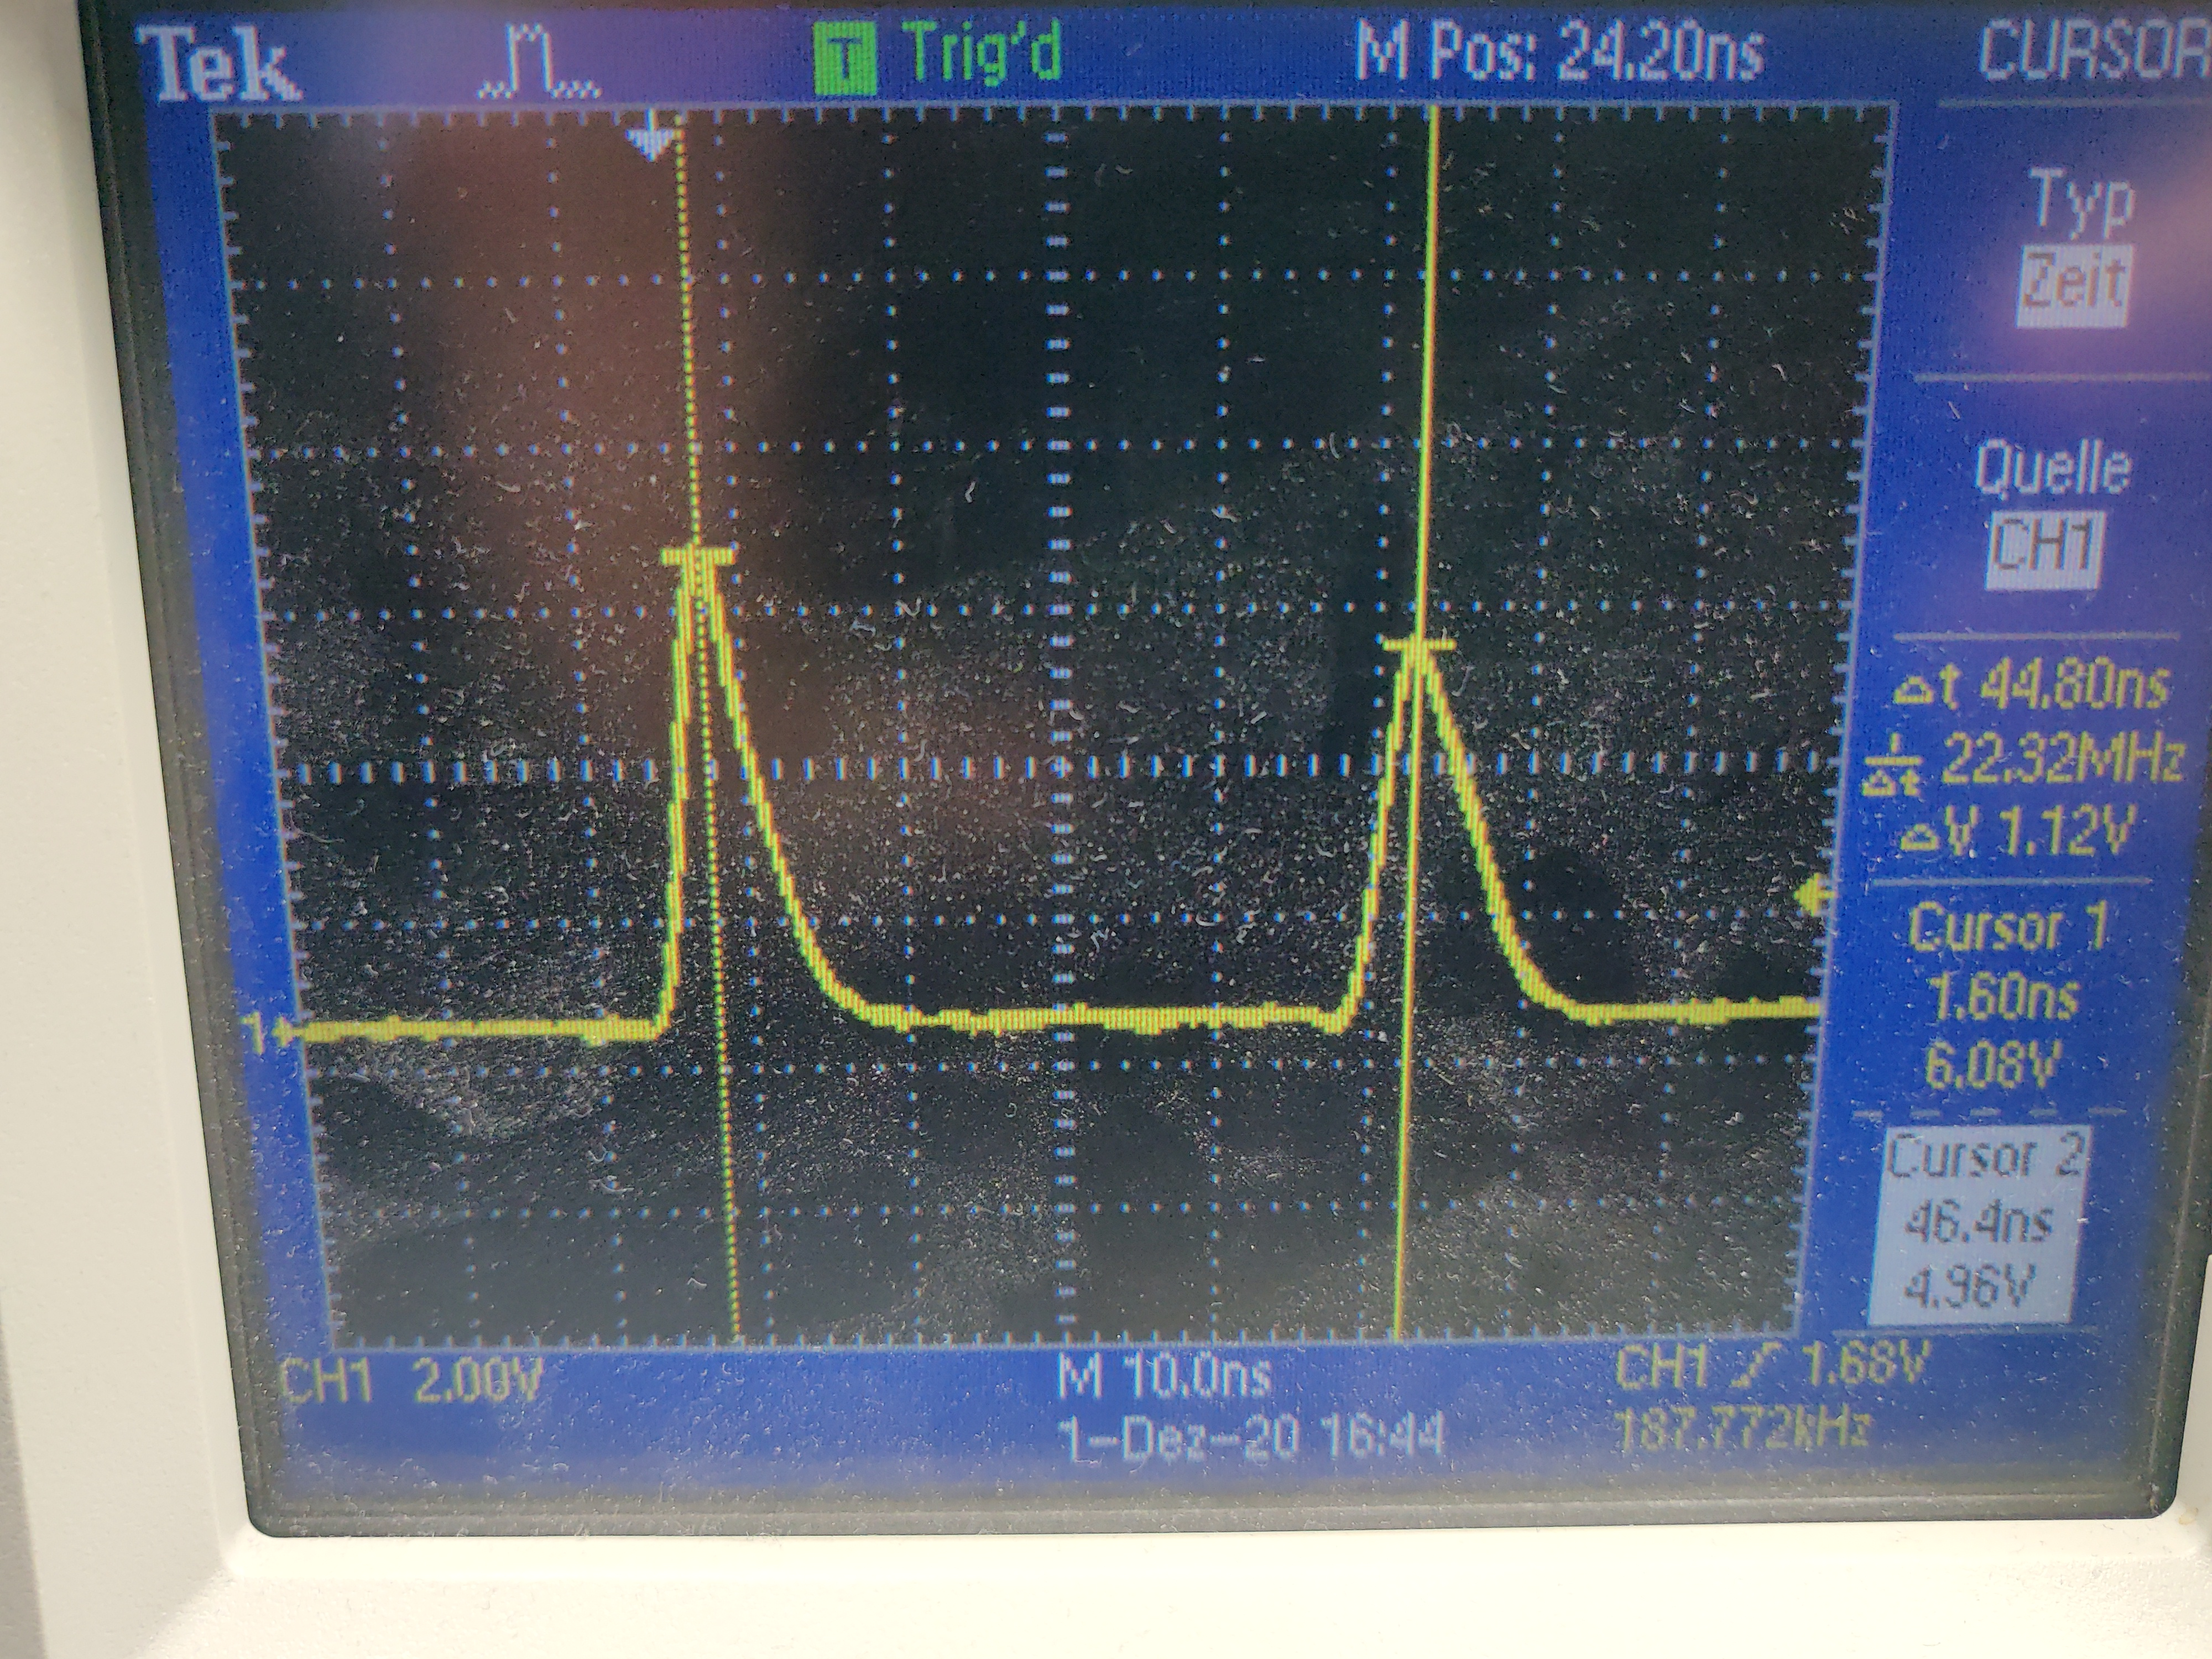
\includegraphics[width=0.45\linewidth]{messdaten/3-3-2_open_reflectionTime.jpg}}\\%
    \subfloat[If the transmission line gets terminated with an impedance close to zero, the reflected pulse gets inverted.\label{subfig:osci:3-3-2_shorted}]
    {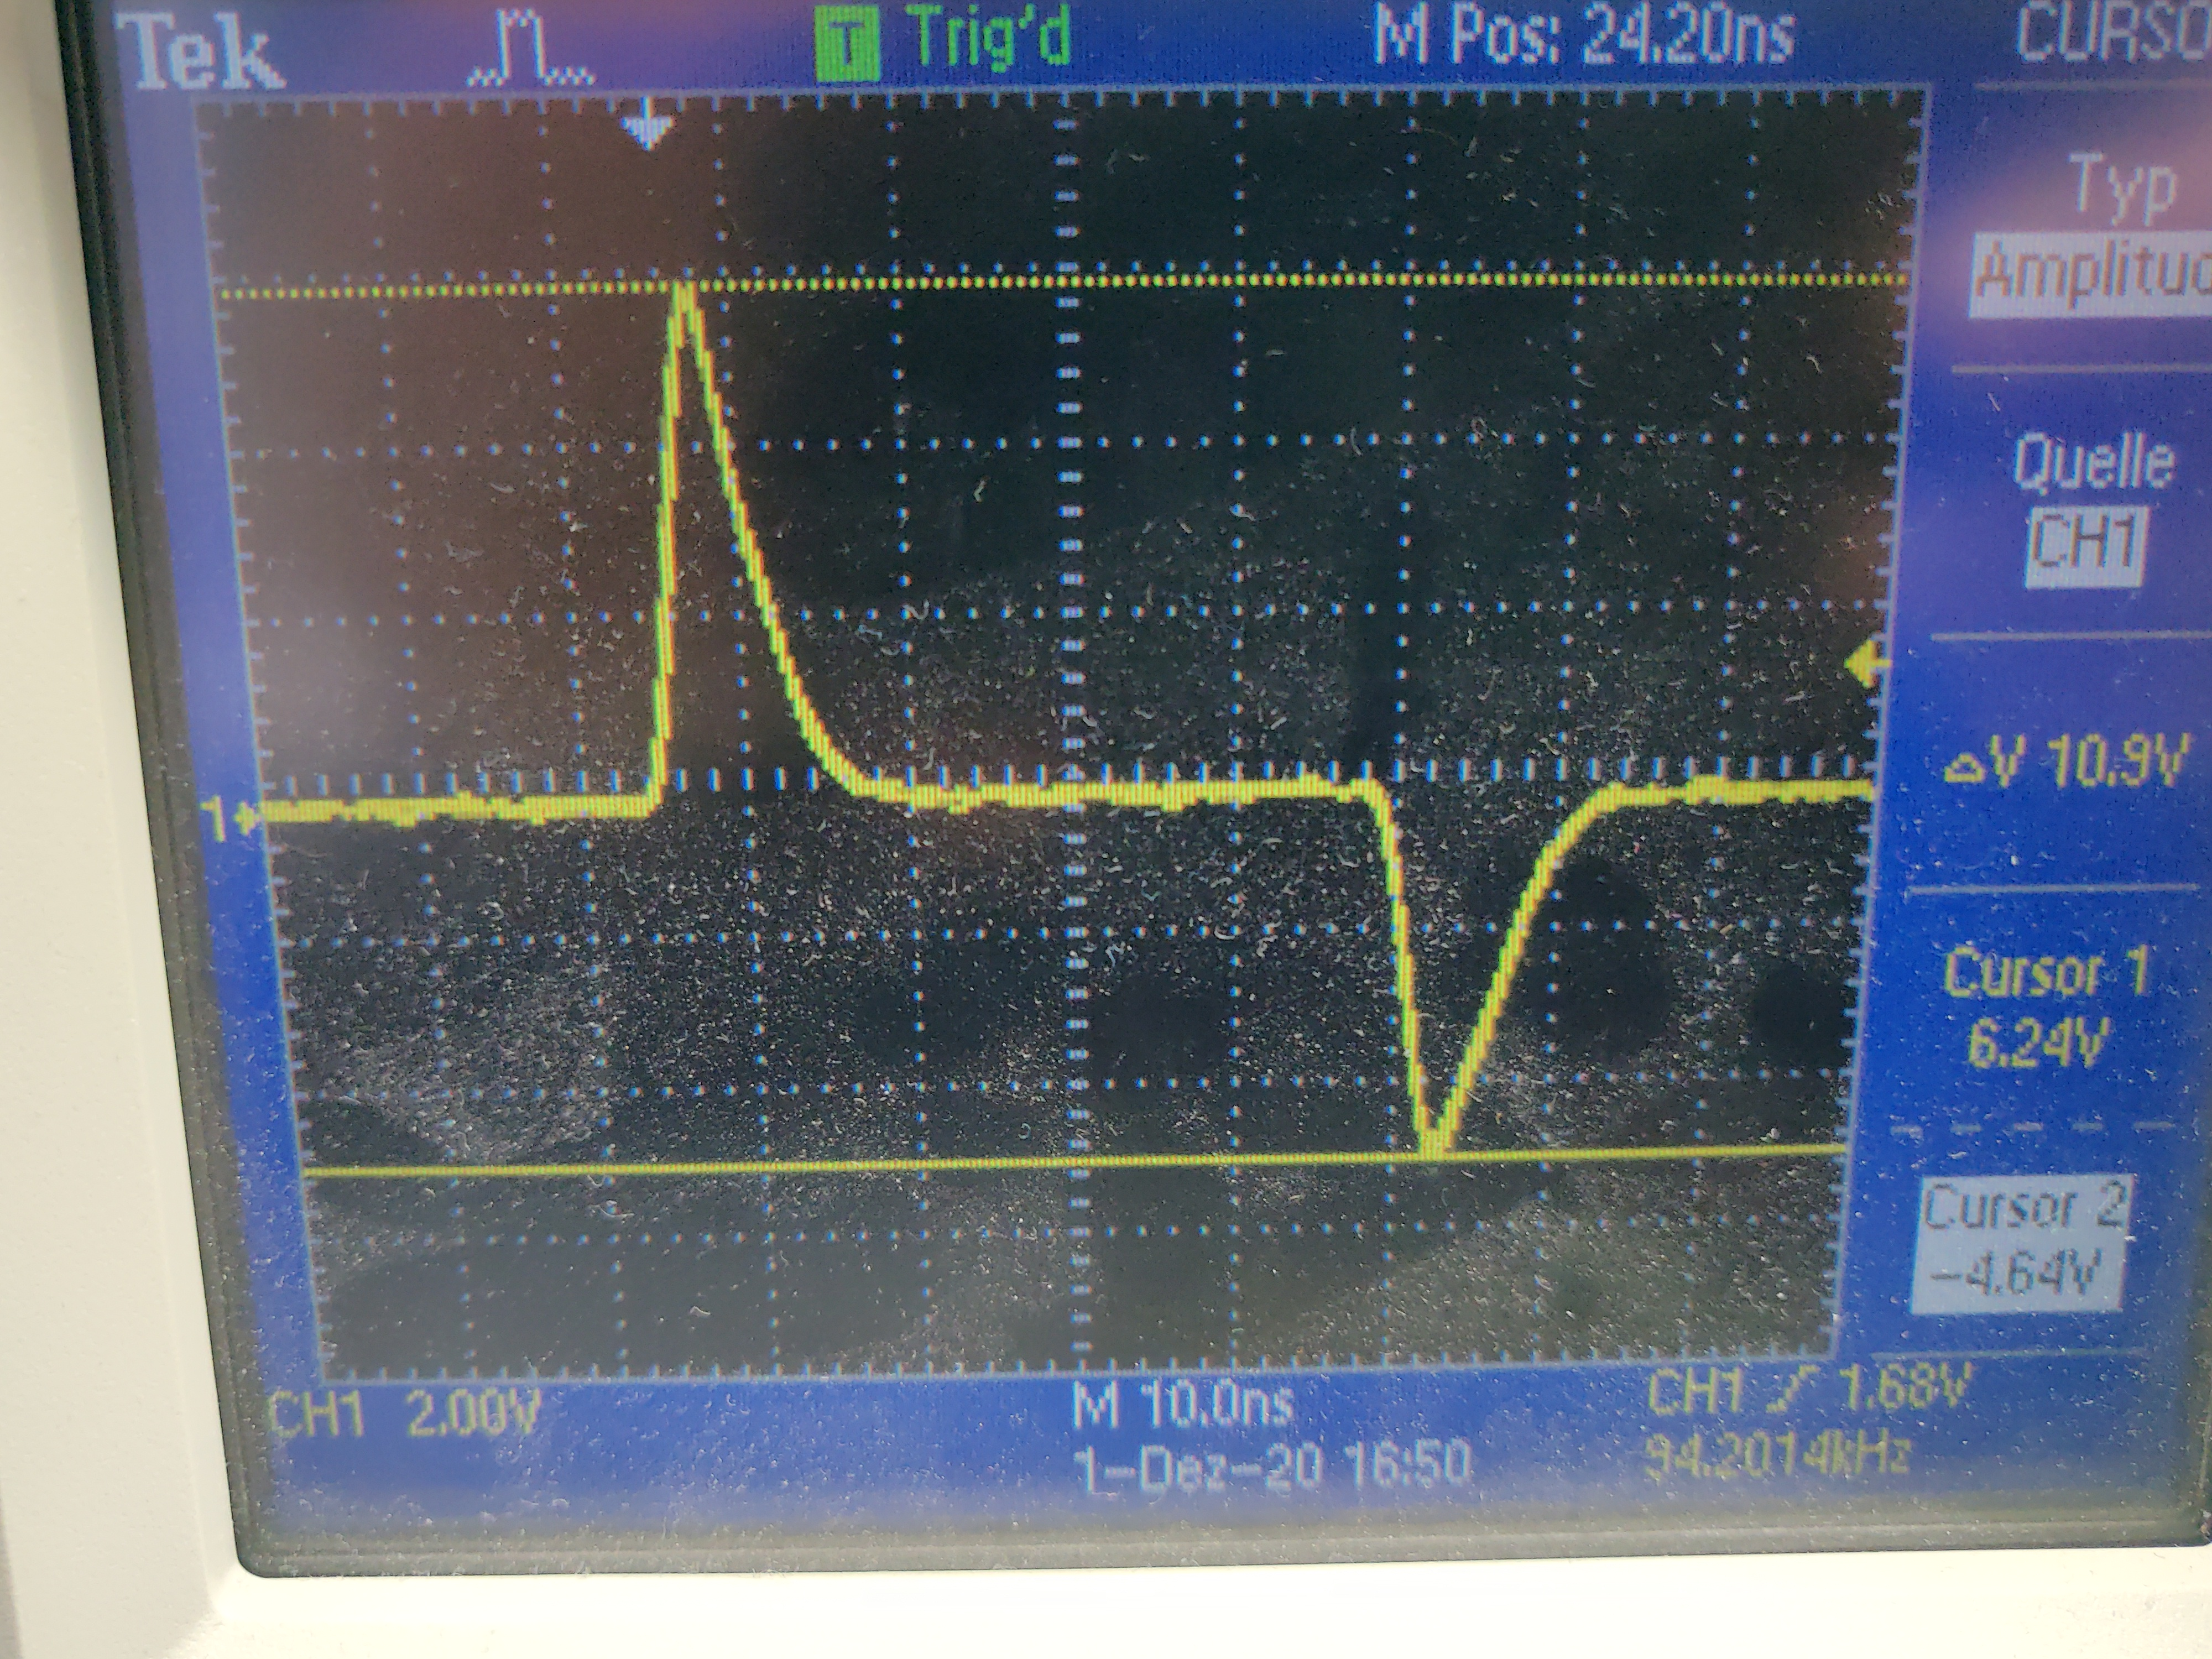
\includegraphics[width=0.45\linewidth]{messdaten/3-3-2_shorted.jpg}}%
    \hspace{.05\linewidth}
    \subfloat[The reflected signal can almost completely inhibited terminating the transmission line with an impedance close to its characteristic impedance.\label{subfig:osci:3-3-2_Z_0_equal_R_term}]
    {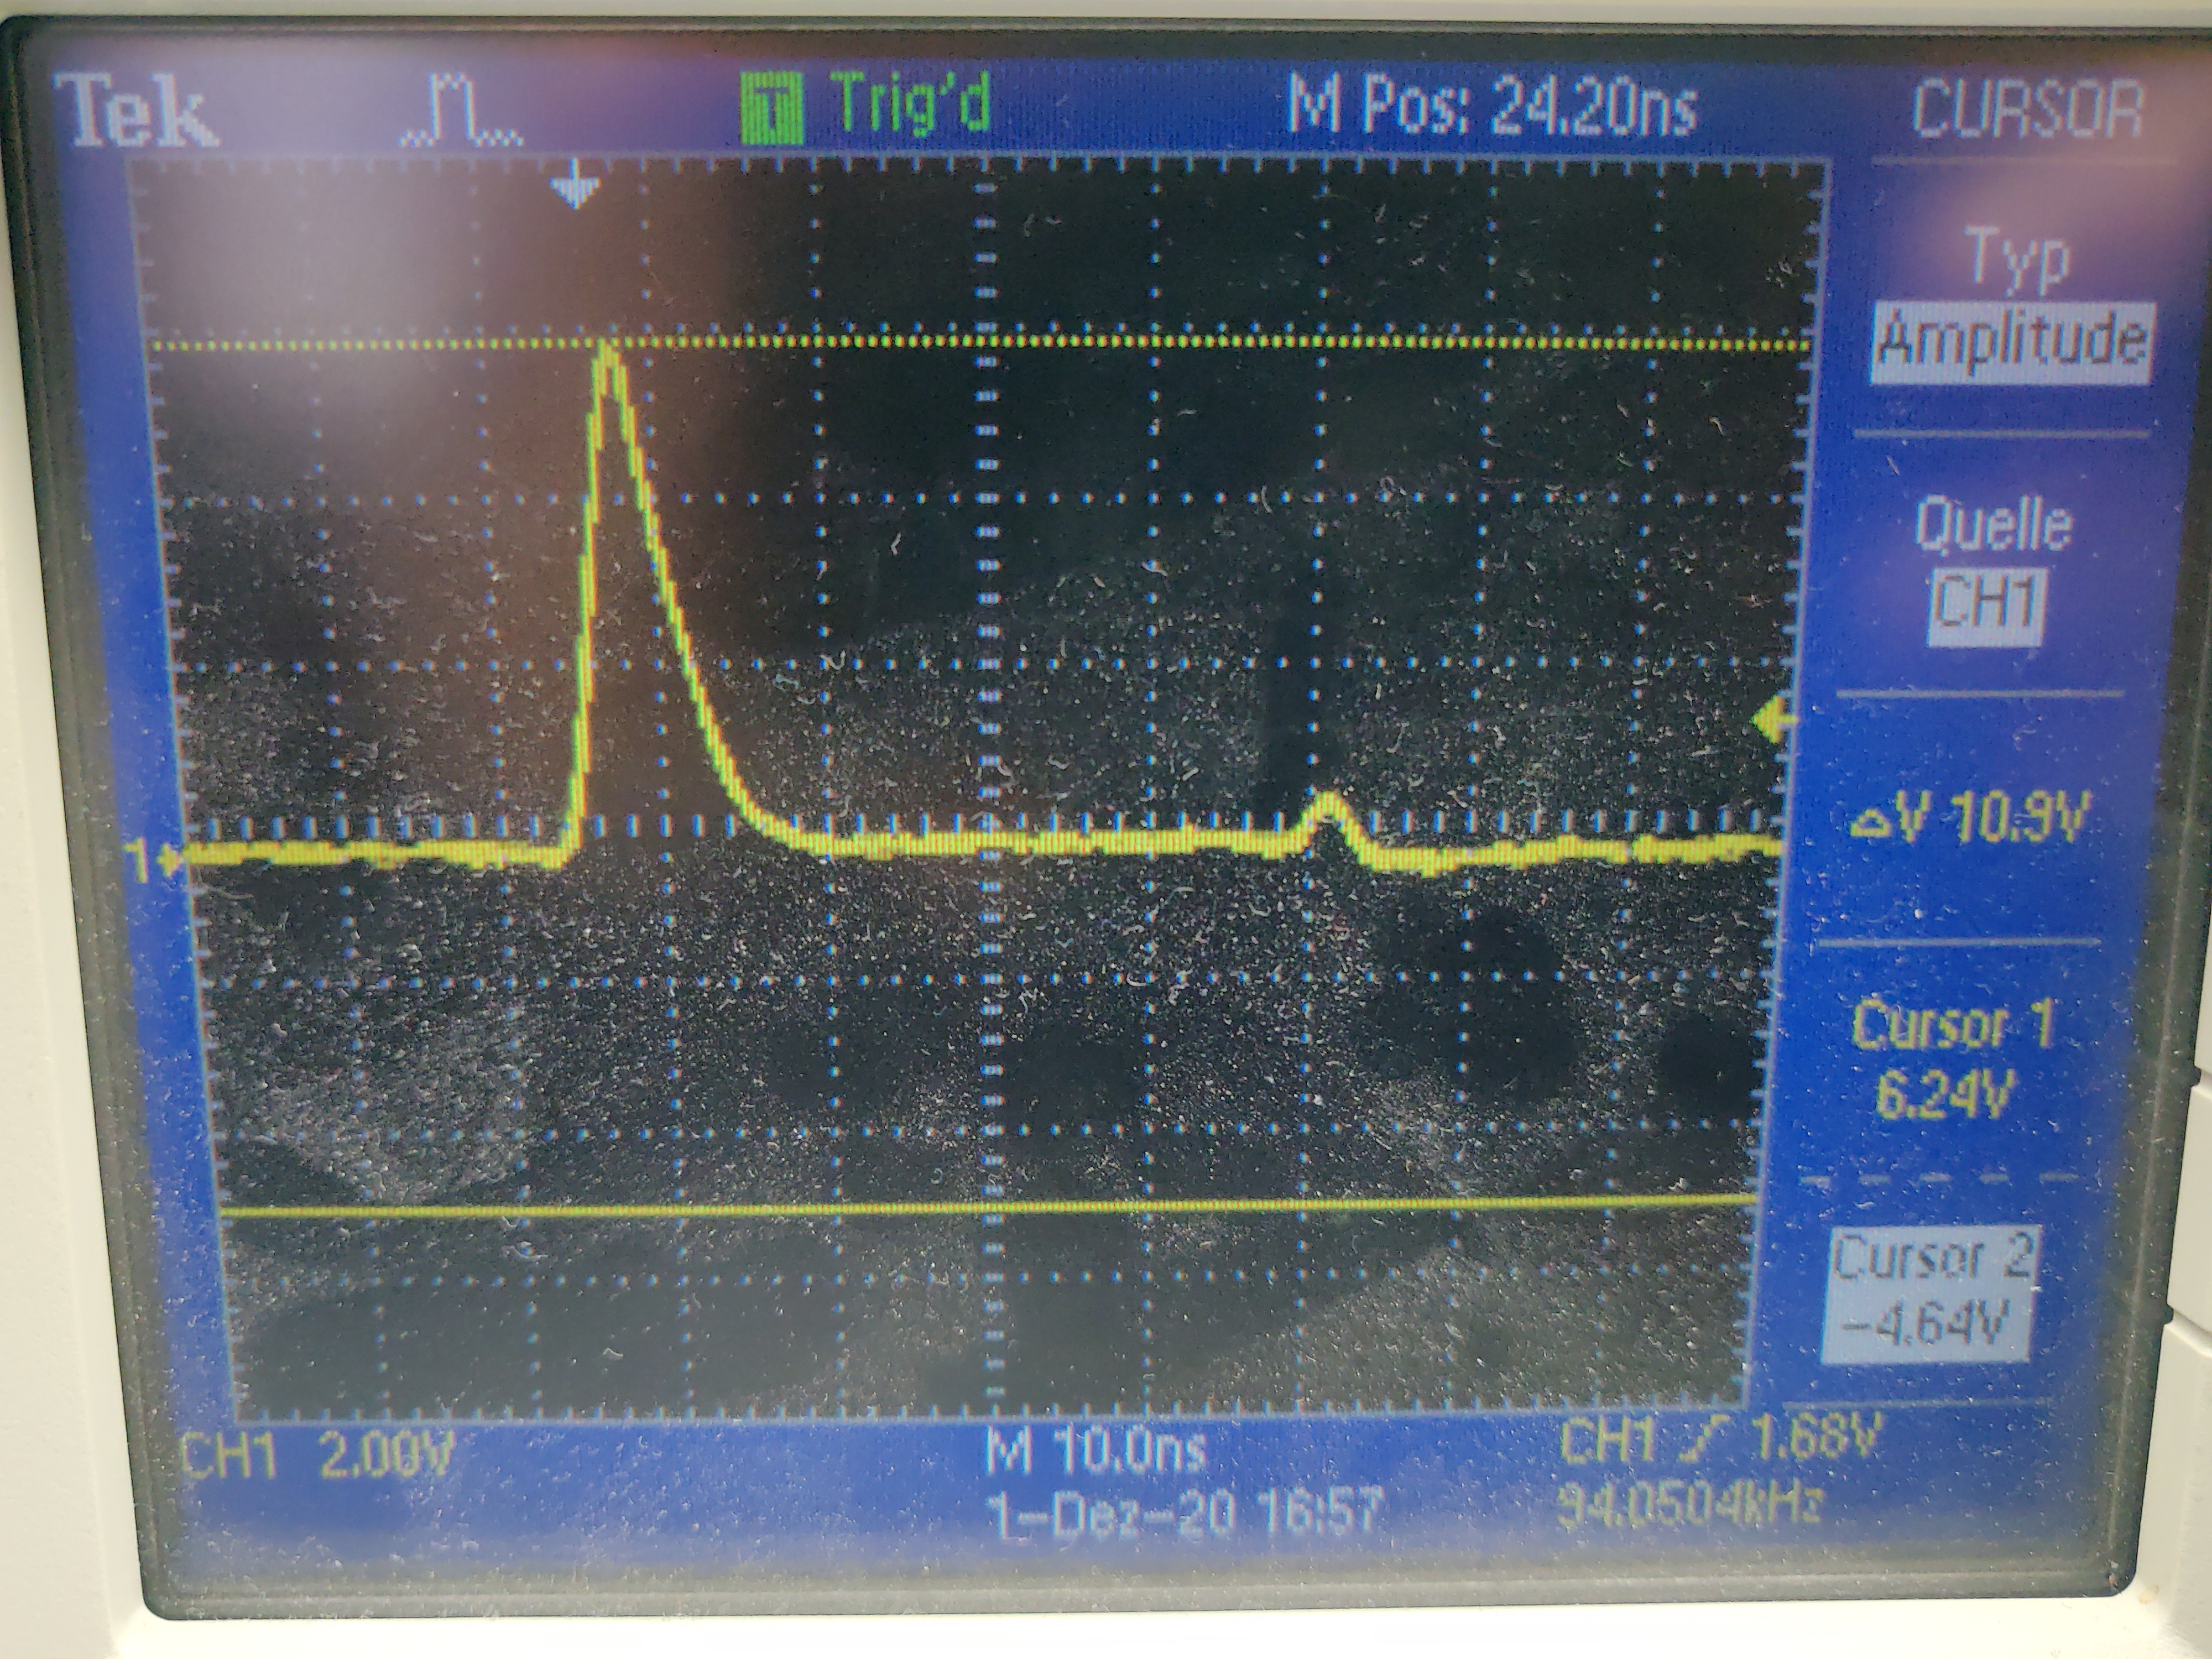
\includegraphics[width=0.45\linewidth]{messdaten/3-3-2_Z_0_equal_R_term.jpg}}%
\end{figure}
\begin{figure}[h]
    \ContinuedFloat%
    \subfloat[Local changes to the cables characteristics reflect signals as well. This can be utilized to locate a defect along the cable's length.\label{subfig:osci:3-3-3_lengthToDefect}]
    {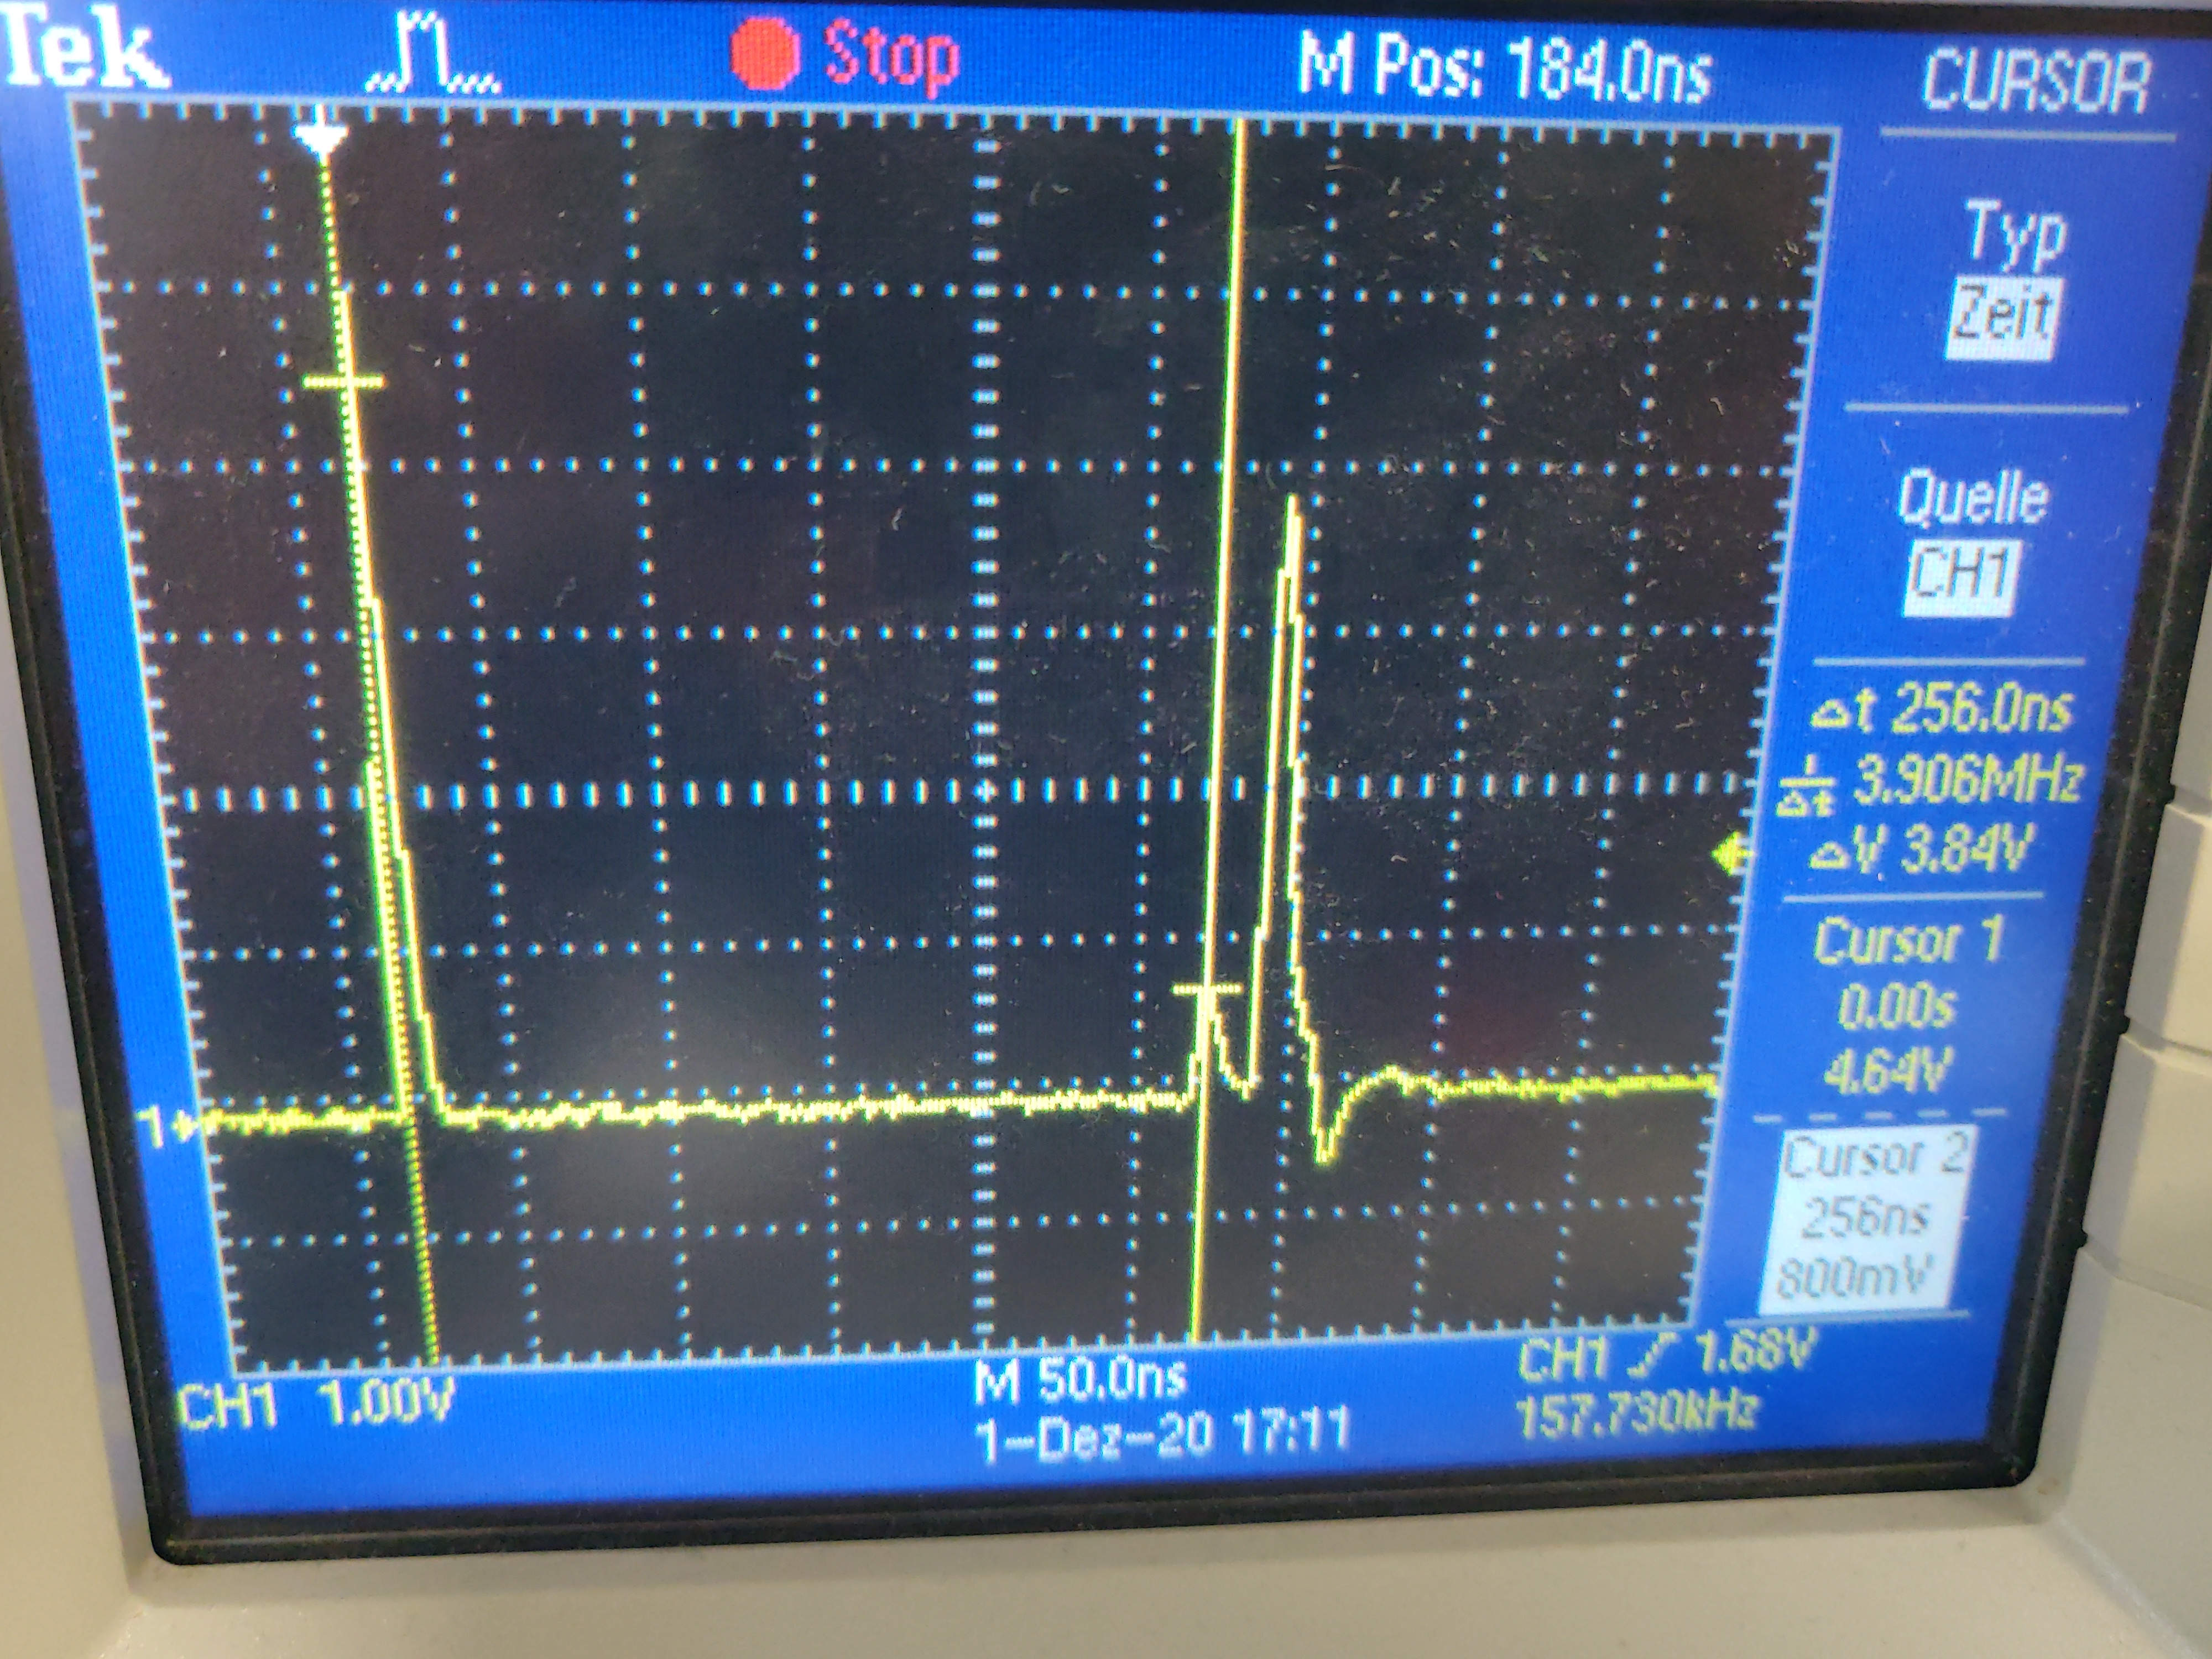
\includegraphics[width=0.45\linewidth]{messdaten/3-3-3_lengthToDefect.jpg}}%
    \hspace{.05\linewidth}
    \subfloat[The length of a transmission line can be deducted by the property of a signal traversing the transmission line at a finite and unaltered speed.\label{subfig:osci:3-3-3_overallLength}]
    {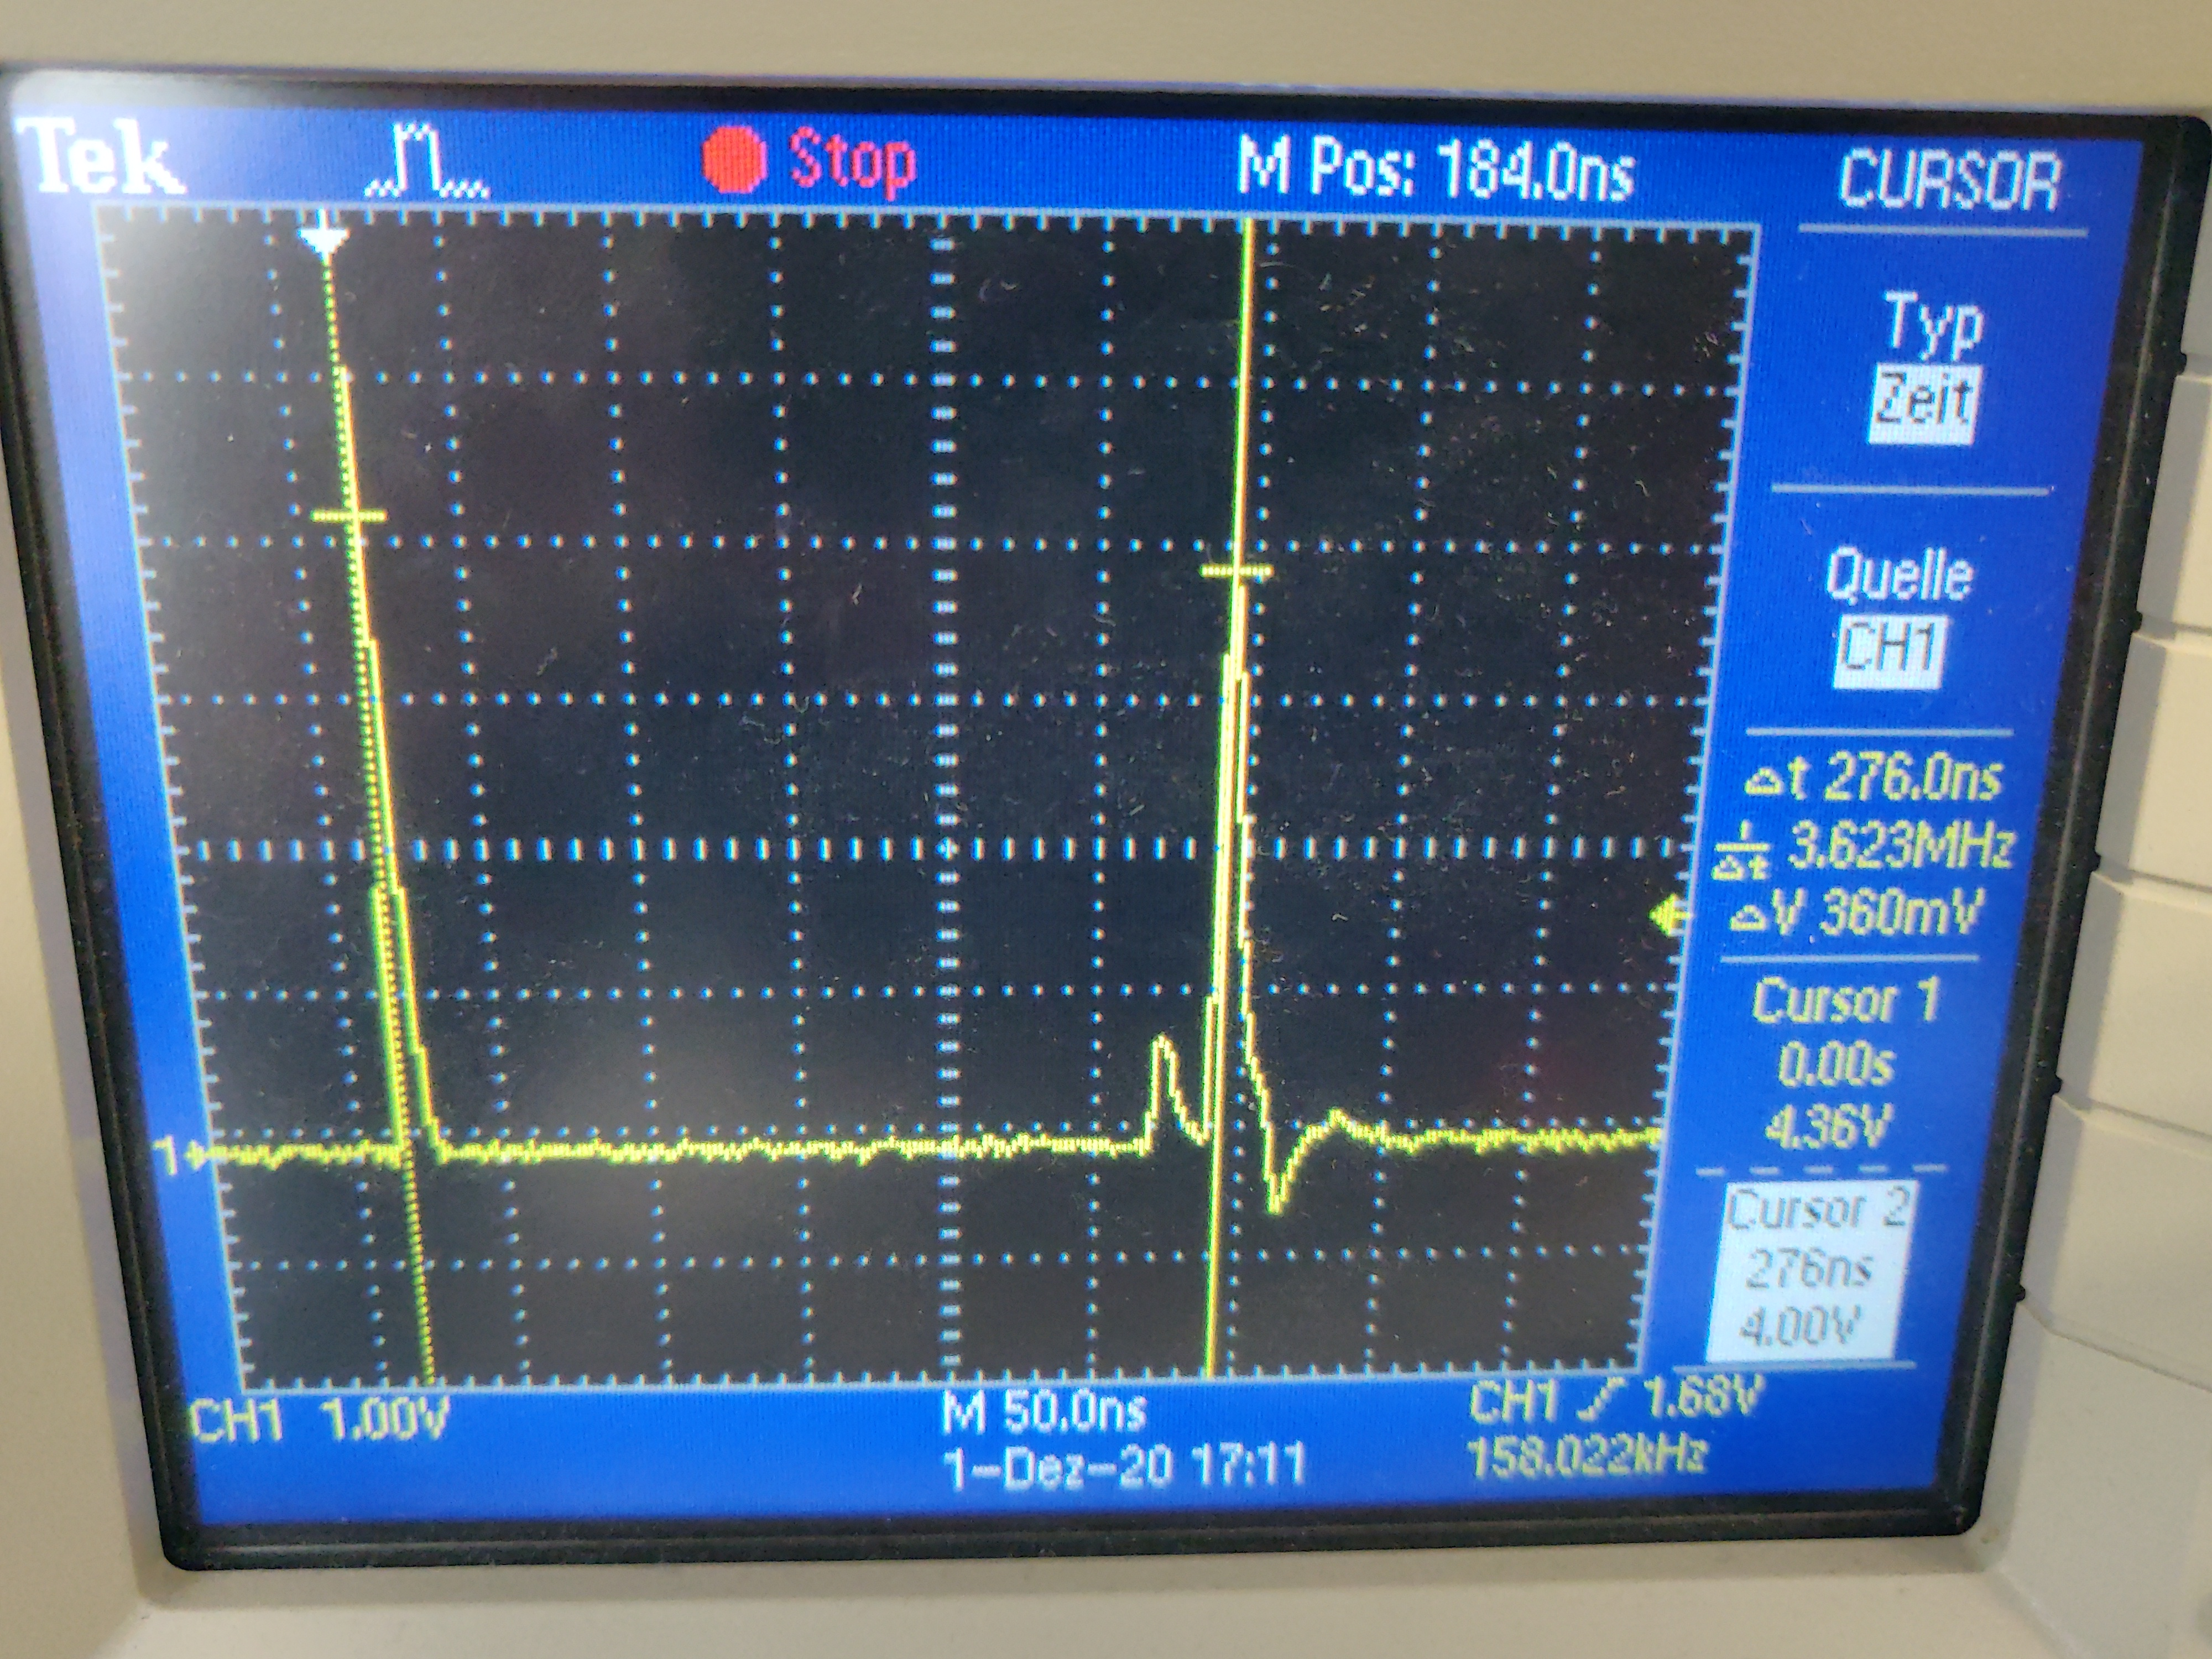
\includegraphics[width=0.45\linewidth]{messdaten/3-3-3_overallLength.jpg}}\\%
    \subfloat[Avalanche pulse signal at $ U_{min} $.\label{subfig:osci:avalanche_pulse_signal}]{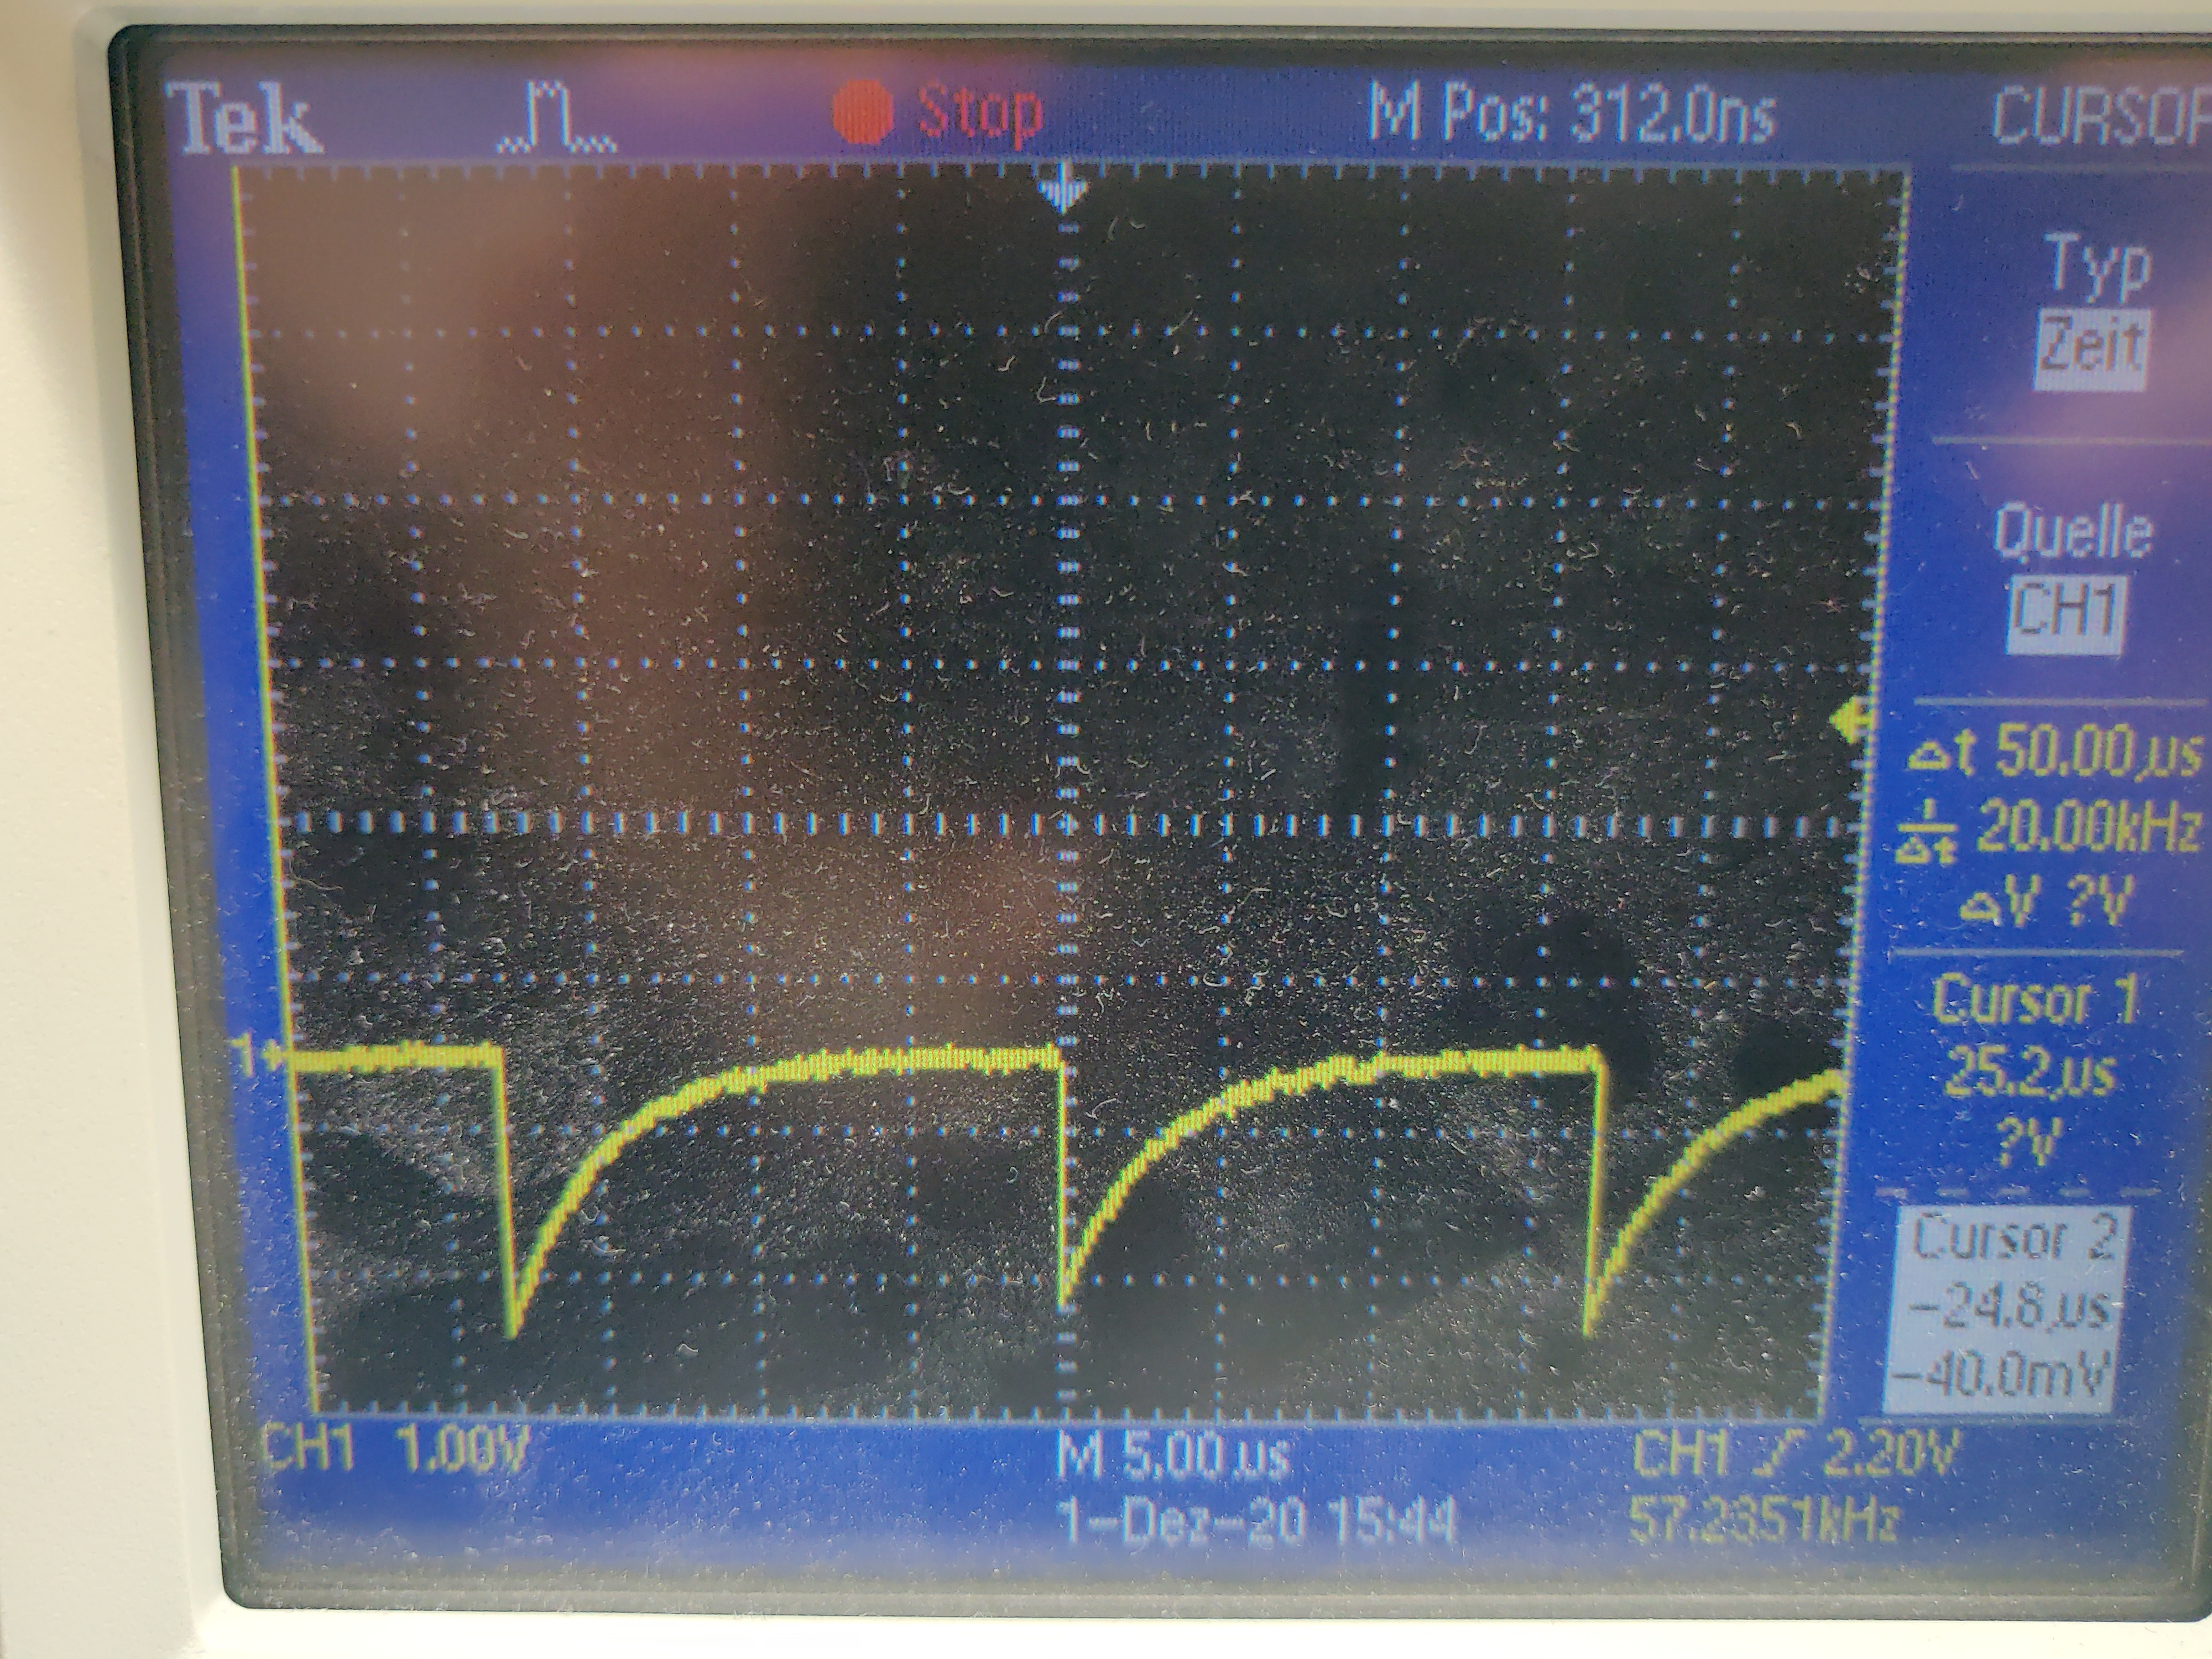
\includegraphics[width=0.45\linewidth]{messdaten/avalanche_pulse_signal.jpg}}%
    \hspace{.05\linewidth}
    \subfloat[Pulse characteristics.\label{subfig:osci:pulsuntersuchung}]{\includegraphics[width=0.45\linewidth]{messdaten/pulsuntersuchung.jpg}}%
    \caption[Oscillograms]{During the course of the experiment captured oscillograms.}%
\end{figure}
%
\begin{figure}
    \centering
    \includesvg[inkscapelatex=false, width=.8\textwidth]{Spice/pulse_attenuation/pulse_attenuation_sim_circuit}
    \caption[\textsc{LTspice} circuit diagram to simulate low-pass behavior]{\textsc{LTspice} circuit diagram to simulate low-pass behavior.}
    \label{fig:pulse_attenuation_sim_circuit}
\end{figure}
%
\newpage
%
\begin{table}[]
    \centering
    \caption[Handwritten notes]{Handwritten notes corresponding each measurement.}%
    \begin{tabular}{cc}
        \adjustbox{valign=t}{
            \subfloat[Duty cycles and measured output voltages at the BC.\label{subtab:3-1_duty_vs_voltage}]{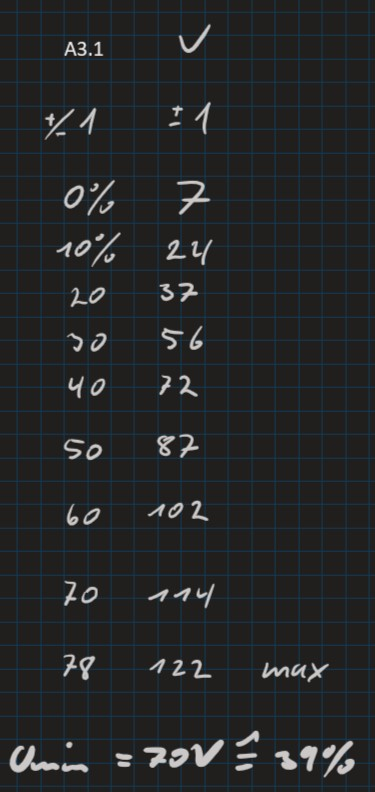
\includegraphics[width=.4\linewidth]{messdaten/handwritten/3-1.jpg}}
            \hspace{.1\linewidth}
        }
        &
        \adjustbox{valign=t}{
            \subfloat[Repetition frequency \( f_{Rep} \) vs. various output voltages.\label{subtab:3-2_duty_vs_repetitionfreq}]{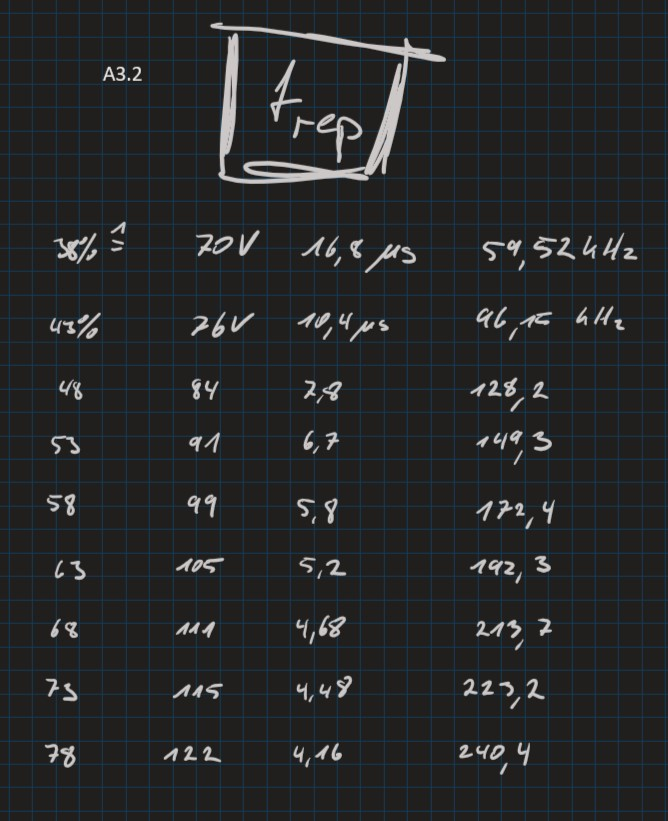
\includegraphics[width=.4\linewidth]{messdaten/handwritten/3-2.jpg}}
            \hspace{.1\linewidth}
        }
    \end{tabular}
\end{table}
\begin{table}[]
    \ContinuedFloat
    \centering
    \begin{tabular}{cc}
        \adjustbox{valign=t}{
            \subfloat[Propagation times at three different cable lengths.\label{subtab:3-3-1_propagationTimes_3_cables}]{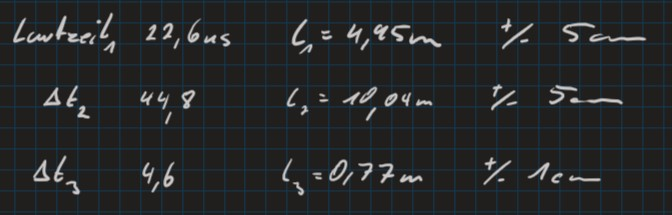
\includegraphics[width=0.4\textwidth]{messdaten/handwritten/3.3.1_propagationTimes.jpg}}%
            \hspace{.1\linewidth}
        }
        &
        \adjustbox{valign=t}{
            \subfloat[Measured impedance of the cables.\label{subtab:3.3.2_cableImpedances}]{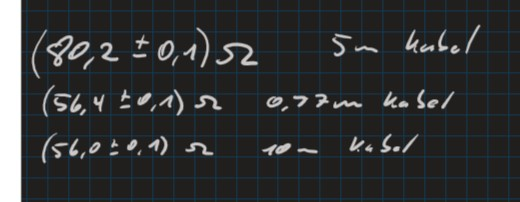
\includegraphics[width=0.4\textwidth]{messdaten/handwritten/3.3.2_cableImpedances.jpg}}%
            \hspace{.1\linewidth}
        }
    \end{tabular}
\end{table}
\begin{table}[]
    \ContinuedFloat
    \centering
    \subfloat[Table of the measured cable characteristics.\label{subtab:3.3.2_cableCharacteristicsTable}]{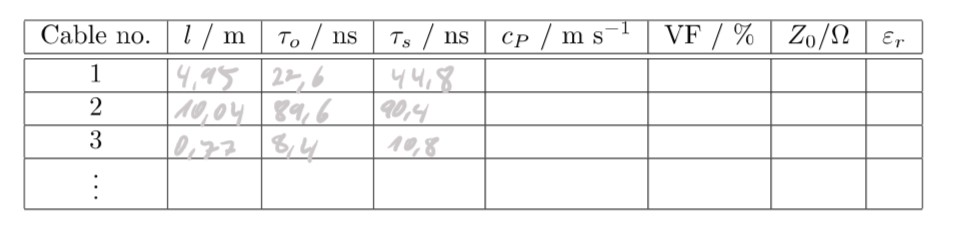
\includegraphics[width=0.6\linewidth]{messdaten/handwritten/3.3.2_cableCharacteristicsTable.jpg}}
\end{table}